\documentclass{standalone}
\usepackage{tikz}

\usetikzlibrary{arrows.meta}

\begin{document}
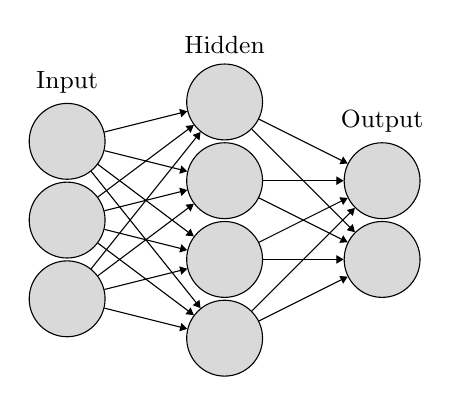
\begin{tikzpicture}
  [neuron/.style={circle,draw,fill=black!15}]
  \node[neuron] (i1) at (0,-0.5) {$\qquad$};
  \node[above,node font=\small] (Input) at (0,0) {Input};
  \node[neuron] (i2) at (0,-1.5) {$\qquad$};
  \node[neuron] (i3) at (0,-2.5) {$\qquad$};

  \node[neuron] (h1) at (2,0) {$\qquad$};
  \node[above,node font=\small] (Hidden) at (2,0.5) {Hidden};
  \node[neuron] (h2) at (2,-1) {$\qquad$};
  \node[neuron] (h3) at (2,-2) {$\qquad$};
  \node[neuron] (h4) at (2,-3) {$\qquad$};

  \node[above,node font=\small] (Output) at (4,-0.5) {Output};
  \node[neuron] (o1) at (4,-1) {$\qquad$};
  \node[neuron] (o2) at (4,-2) {$\qquad$};
  
  \foreach \from/\to in {
    i1/h1,i1/h2,i1/h3,i1/h4,
    i2/h1,i2/h2,i2/h3,i2/h4,
    i3/h1,i3/h2,i3/h3,i3/h4,
    h1/o1,h1/o2,
    h2/o1,h2/o2,
    h3/o1,h3/o2,
    h4/o1,h4/o2}
  \path (\from) edge [arrows = {-Stealth[inset=0pt, angle=60:3pt]}] (\to);
\end{tikzpicture}
\end{document}
%%% Local Variables:
%%% mode: latex
%%% TeX-master: t
%%% End:
